%--------------------------------------------------------------------------------
\chapter{Error estimation}\label{sec:error_estimation}
In this section a Fourier mode analysis for constant $\Dx$ and $\Psi$ of \autoref{eq:1d_regularization} is given.
For convenience the equation is repeated here:
%
\begin{align}
    \widetilde u - \pdiff{}{x}  \Psi \pdiff{\widetilde u}{x} = u_{\it{giv}}
\end{align}

The Fourier-mode transform of \autoref{eq:1d_regularization} reads, when $\Dx = \it{constant}$ and $\Psi = c_{\Psi} \Dx^2 = \it{constant}$:
\begin{align}
\widetilde u \exp(\ii k x) \left( 1 + \Psi k^2 \right) = \mathcal{F}(u_{giv})
\end{align}
multiply $\Psi$ by $\Dx^2/\Dx^2 = 1$ yields
\begin{align}
\widetilde u \exp(\ii k x) \left( 1 + \frac{\Psi}{\Dx^2} (k\Dx)^2 \right) = \mathcal{F}(u_{giv})
\label{eq:F_regularization}
\end{align}
which is easier to use in the analysis due to the term $k\Dx$.

The discretisation of \autoref{eq:disc_regularization} with constant $\Dx$ and $\Psi$ yields:
\begin{align}
\left( \frac{1}{8}
- c_{\Psi} \right)  u_{i-1}
+ \left( \frac{6}{8} + 2c_{\Psi}\right)  u_i & +
\left(  \frac{1}{8} - c_{\Psi} \right)  u_{i+1}  =
\\
& = \frac{1}{\Dx}\int_{x_{i-1/2}}^{x_{i+\half}} u_{giv}\, dx
\end{align}
% If \Psi is not constant
%\begin{align}
%    \left( \frac{1}{8}
%    - \frac{\Psi_{i-1} + \Psi_{i}}{2} \right)  u_{i-1}
%    + \left( \frac{6}{8} + \frac{\Psi_{i-1} + 2\Psi_{i} + \Psi_{i+1}}{2}\right)  u_i & +
%     \left(  \frac{1}{8} - \frac{\Psi_{i} + \Psi_{i+1}}{2} \right)  u_{i+1}  =
%     \\
%     & = \frac{1}{\Dx}\int_{x_{i-1/2}}^{x_{i+\half}} u_{giv}\, dx
%\end{align}

Substitution of the Fourier modes
\begin{align}
\overline u_k =  \overline u_k \exp(\ii k \Dx)\quad \text{and} \quad  u_{giv} = u_{giv,k} \exp(\ii k \Dx)
\end{align}
in this equation yields:
\begin{align}
\overline u_k  \left(  \left( \frac{1}{8} -  c_{\Psi}\right) \exp(-\ii k \Dx) +
\left(\frac{6}{8} + 2c_{\Psi} \right) +
\left( \frac{1}{8} -  c_{\Psi} \right) \exp(-\ii k \Dx) \right)  = &
\\
= \frac{u_{giv,k}}{\Dx} \int_{x_{i-1/2}}^{x_{i+\half}}  \exp(\ii k \Dx)\, dx &
\end{align}
$\Rightarrow$
\begin{multline}
\overline u_k \left(  \frac{6}{8} + 2c_{\Psi} + \left( \frac{1}{8} -  c_{\Psi} \right)  2 \cos(k\Dx) \right)
=
\\
= u_{giv,k} \frac{-\ii (\exp(\frac{\ii}{2} k \Dx) - \exp(\frac{\ii}{2} k \Dx) )}{k\Dx}
\end{multline}
$\Leftrightarrow$
\begin{multline}
\overline u_k \left(  \frac{6}{8} + 2c_{\Psi} + \left( \frac{1}{8} -  c_{\Psi} \right)  2 \cos(k\Dx) \right)
= u_{giv,k} \frac{2 \sin(\half k \Dx)}{k\Dx}
\label{eq:regularize_piecewise_linear}
\end{multline}

The ratio between the regularized function $\widetilde{u}$ (\autoref{eq:F_regularization}) and given function reads (see \autoref{fig:ratio_func}):
\begin{align}
\widetilde{r} = \abs{  \frac{\widetilde u_k}{ u_{giv,k}} } & = \abs{ \frac{1}{1 + c_{\Psi} (k \Dx)^2} } \label{eq:r_tilde}
\end{align}
and the ratio between the piecewise linear function $\overline{u}$ (\autoref{eq:regularize_piecewise_linear}) and given function reads (see \autoref{fig:ratio_func}):
\begin{align}
\overline{r} = \abs{  \frac{\overline u_k}{ u_{giv,k}} } & = \abs{ \frac{2 \sin(\half k \Dx)}{k\Dx\left( \frac{6}{8} + 2c_{\Psi} + \left( \frac{1}{8} -  c_{\Psi} \right)  2 \cos(k\Dx) \right)} }
\end{align}
$\Leftrightarrow$
\begin{align}
\overline{r} = \abs{  \frac{\overline u_k}{ u_{giv,k}} } & = \abs{ \frac{8 \sin(\half k \Dx)}{k\Dx\left( 3 + \cos(k\Dx) + 8c_{\Psi} ( 1 - \cos(k\Dx))\right) } }
\end{align}

\begin{figure}[H]
\centering
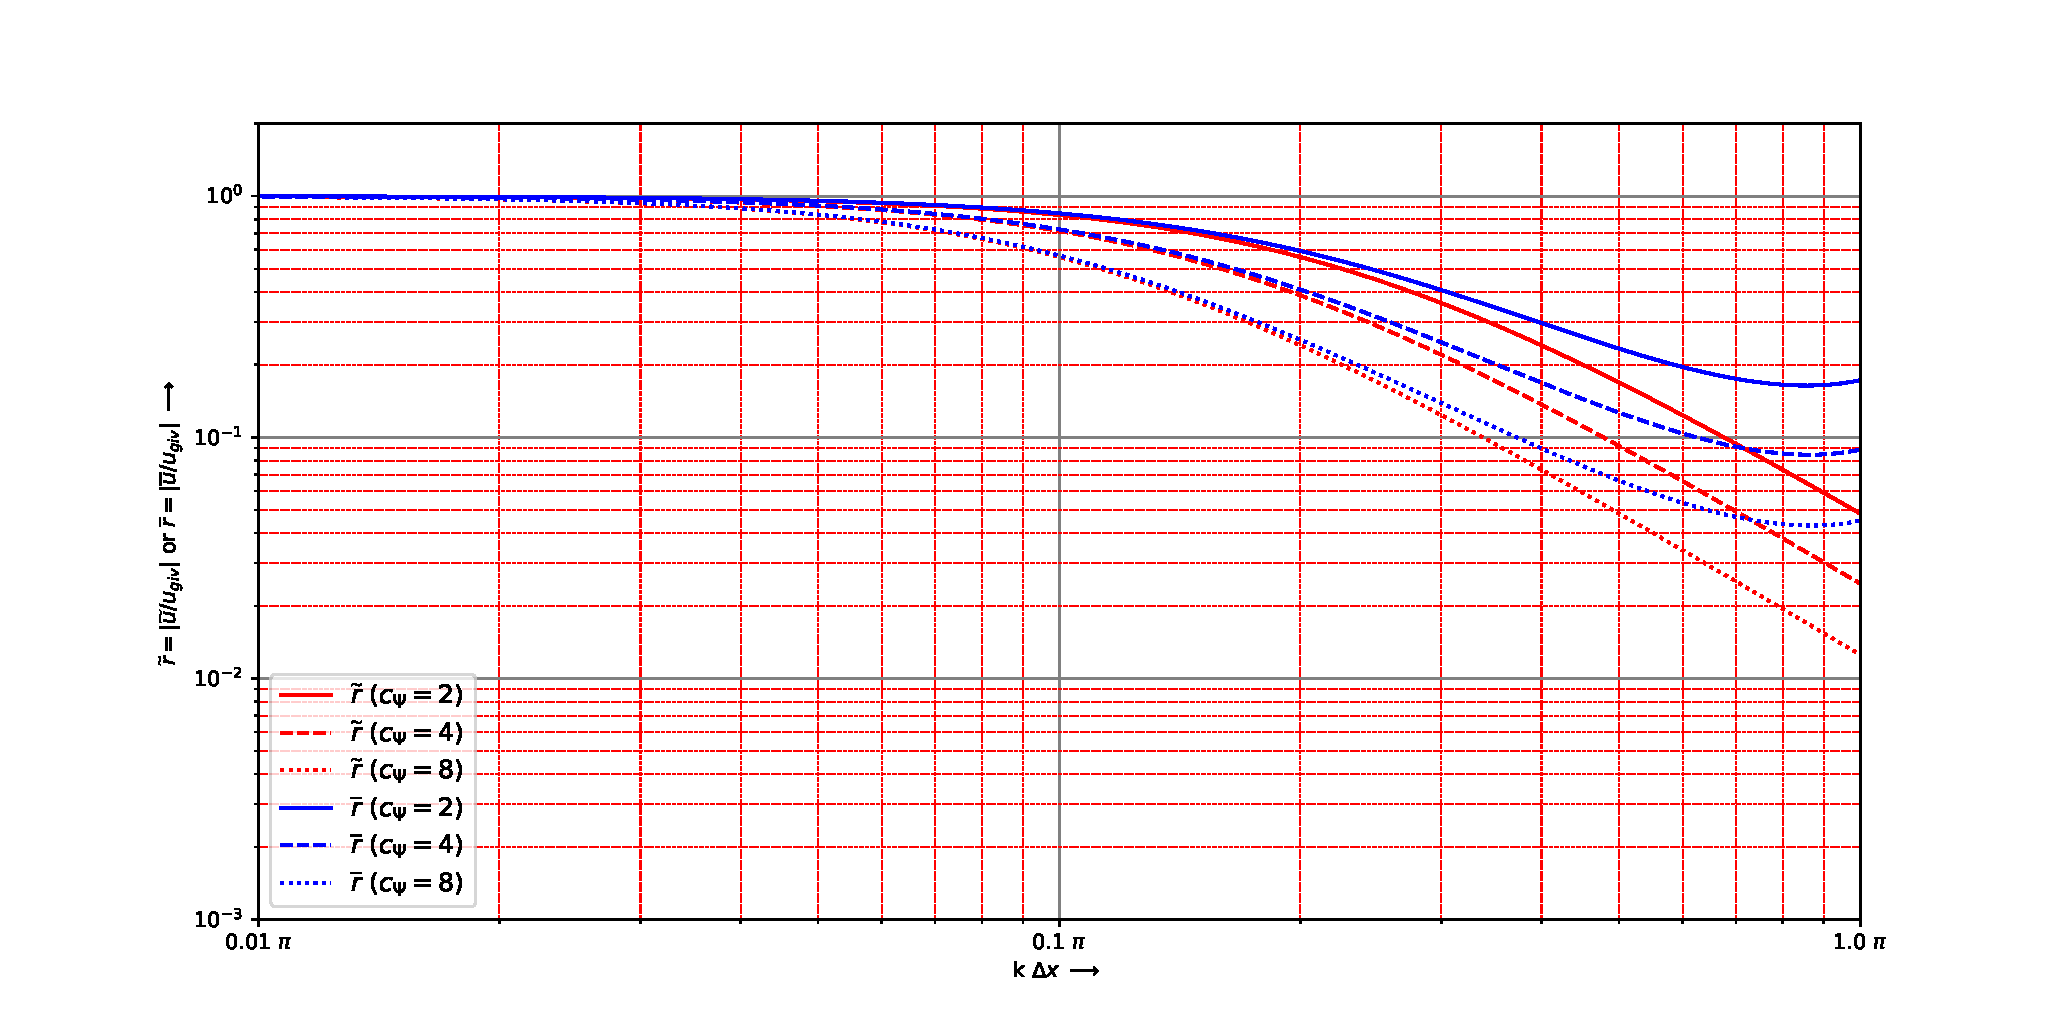
\includegraphics[width=0.99\textwidth]{figures/ratio_u_u_giv.pdf}
\caption{Ration between $\widetilde{r} = \abs{\widetilde{u}_k/u_{giv,k}}$ , and $\overline{r} = \abs{\overline{u}_k/u_{giv,k}}$. For different values of $c_{\Psi} = \Psi/\Dx^2$.\label{fig:ratio_func}}
\end{figure}
%--------------------------------------------------------------------------------
\section{Numerical error}
Discretization error values are determined when  $\Dx = {\it constant} $ and $\Psi = 0$, \autoref{eq:disc_regularization} reduces to:
\begin{align}
\frac{1}{8}      u_{i-1}
+ \frac{6}{8}   u_i
+ \frac{1}{8}   u_{i+1}  = \frac{1}{\Dx} \int_{x_{i-1/2}}^{x_{i+\half}} u_{giv}\, dx
\label{eq:disc_regularization_psi_0}
\end{align}

Numerical error as discretized between grid pints
\begin{align}
{\text{errorFVEgridpoint}}(k\Dx) = \abs{  1- \frac{8 \sin(\half  k\Dx)}{k\Dx  (3 + \cos(k\Dx))}}
\end{align}
Numerical error as discretized between cell centres (numerical Fourier-mode through the cell centres)
\begin{align}
{\text{errorFVEcellcentre}}(k\Dx) & = \abs{ 1 - \frac{8 \sin(\half k\Dx) \cos(\half k\Dx)}{k\Dx (3 + \cos(k\Dx))}}
\end{align}
With lowest order estimation of (see \citet{funcfitsmoothing_Fouriermodeanalysis2024}):
\begin{align}
-\frac{1}{24} (k\Dx)^2 - \frac{7}{960} (k\Dx)^4 + O(\Dx^6) % Computed with MapleSoft
\end{align}

So if the numerical error needs to be smaller then 1\ \%, the number of grid cells per wave length ($\lambda = N\Dx$) is computed as
\begin{align}
\frac{1}{24}(k\Dx)^2 < 0.01 \Rightarrow k\Dx < 0.5 \Rightarrow
\\
\left(\frac{2\pi}{N\Dx}\right)\Dx < 0.5 \Rightarrow N > 4\pi \approx 13
\end{align}
so per wave detail $\approx 7$ grid cells.

Discretization error values are given when  $\Psi = c_{\Psi}\Dx^2 = 0$ (see \autoref{fig:error_func}):
\begin{figure}[H]
\centering
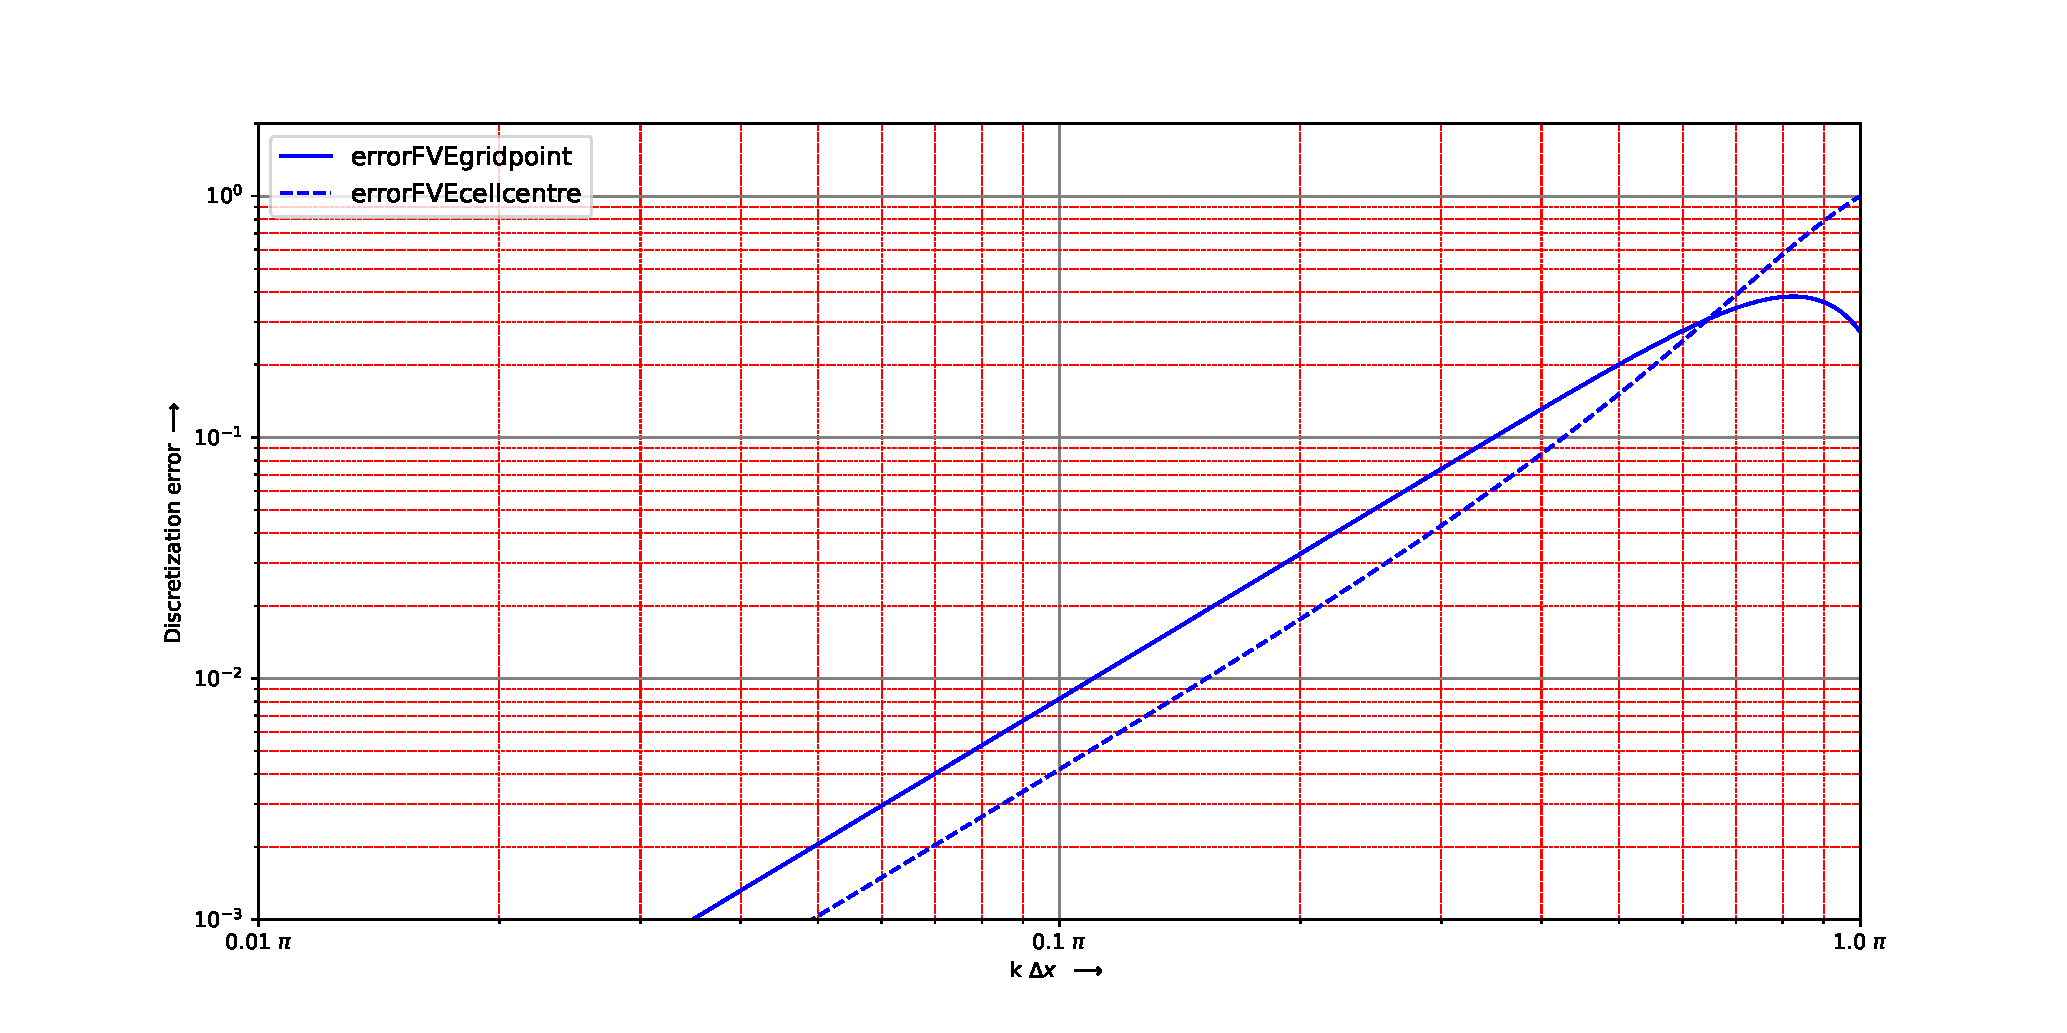
\includegraphics[width=0.99\textwidth]{figures/discr_error_u_u_giv.pdf}
\caption{Error function for value $\Psi = c_{\Psi}\Dx^2 = 0$. \label{fig:error_func}}
% python script: regularization_error_u_giv_u.py
\end{figure}

%-------------------------------------------------------------------------------
\section{Determining the factor $\mathbf{c_{\Psi}}$}\label{sec:determine_factor_c_psi}
In the limit of $k\Dx \rightarrow \infty$ \autoref{eq:r_tilde} behaves as:
\begin{align}
\lim_{k\Dx\to \infty}\frac{1}{1 + c_{\Psi}(k\Dx)^2} = \frac{1}{c_{\Psi}(k\Dx)^2}
\end{align}
The cut-off frequency is determined by $1 = 1/(c_{\Psi} (k\Dx)^2)$, hence filter parameter $c_{\Psi} = 1/(k\Dx)^2$ gives cut-off frequency $k$, or $k\Dx =\sqrt{1/c_{\Psi}}$ is obtained with filter parameter $c_{\Psi}$.
Given the wave length from the required numerical error (1\ \%, $N = 13$), the coefficient $c_{\Psi}$ reads:
\begin{align}
c_{\Psi} = \frac{1}{(k\Dx)^2} \quad \Rightarrow \quad c_{\Psi} = \frac{N^2 }{(2\pi)^2} \approx 4
\end{align}
%
%--- begin light blue table ---
\begin{longtable}{>{\bfseries}p{6mm-12pt}|p{\textwidth/3-2mm-12pt}|p{\textwidth/3-2mm-12pt}|p{\textwidth/3-2mm-12pt}}
\caption{Several typical values for numerical accuracy, $c_{\psi}$ and number of nodes per wavelength ($N$), the highligthed line is set as default.} \\%
 \rowcolor{mgreen1}
& {\textcolor{white}{\textbf{Accuracy}}}
& {\textcolor{white}{$\mathbf{c_{\Psi}}$}}
& {\textcolor{white}{$\mathbf{N}$}}
\\
\topline
\endfirsthead
\endhead
\endfoot
\bottomline
\endlastfoot
1 & 5\ \%   &  0.5 & 4.5\\
\midline
2 & 2\ \%  & 2    & 8.9 \\
\midline
\rowcolor{mgreen2} 3 & 1\ \%  &  4   & 12.8 \\
\midline
4 & 0.5\ \% & 10  & 18.1 \\
\end{longtable}
%--- end light blue table ---
%

%--------------------------------------------------------------------------------
\section{$L^1$-norm for the functions $\widetilde{u}$, $\overline{u}$ and $u_{\it given}$}
The next figures show the $L^1$-norm for the functions
$\abs{|\widetilde{u} - u_{\it giv}|}_{1}$,
$\abs{|\overline{u}  - u_{\it giv}|}_{1}$ and
$\abs{|\overline{u}  - \widetilde{u}|}_{1}$
\begin{figure}[H]
\begin{subfigure}{0.49\textwidth}
    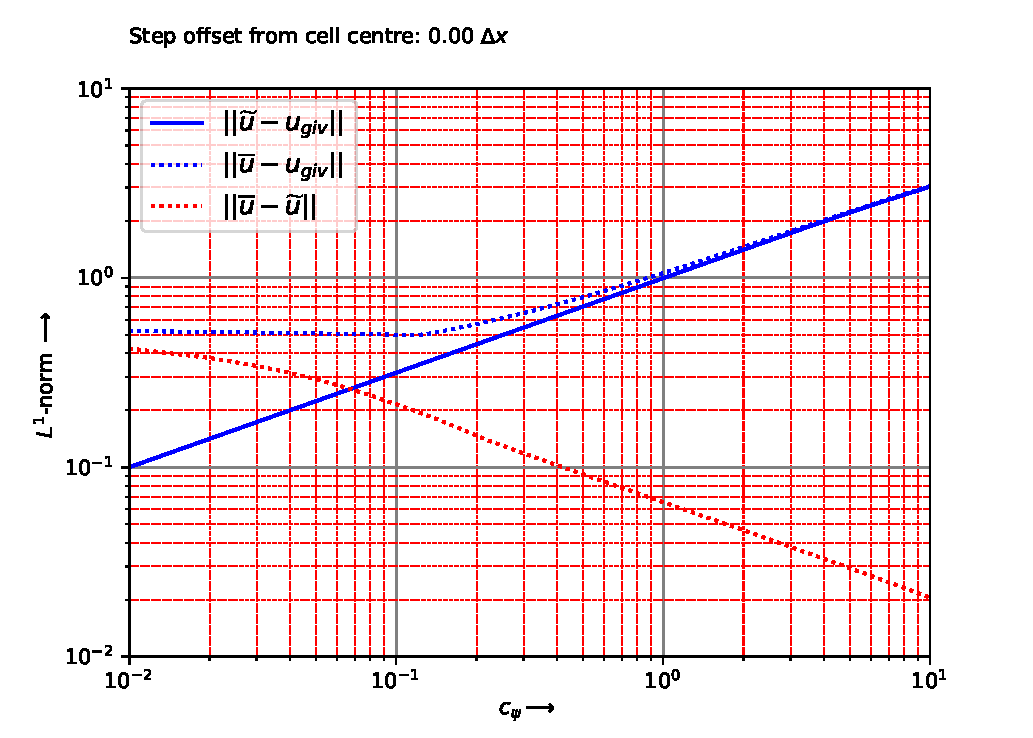
\includegraphics[width=\textwidth]{figures/regul_1d_step_at=0.0_dx50.0.pdf}
    \caption{Step defined at cell centre.\newline\phantom{text}\label{fig:L1_norm_dx_offset_0.0dx}}
\end{subfigure}
\hfill
\begin{subfigure}{0.49\textwidth}
    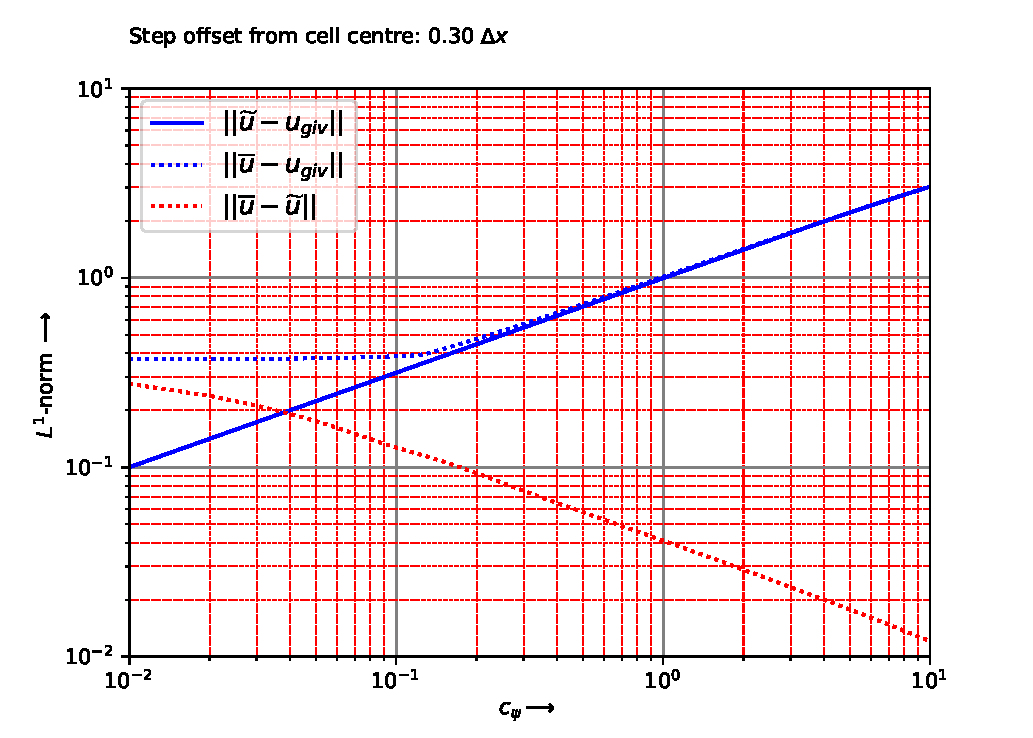
\includegraphics[width=\textwidth]{figures/regul_1d_step_at=0.3_dx50.0.pdf}
    \caption{Step defined with an of set of  0.3 $\Delta x$ from cell centre.\label{fig:L1_norm_dx_offset_0.3dx}}
\end{subfigure}
\\
\begin{subfigure}{0.49\textwidth}
    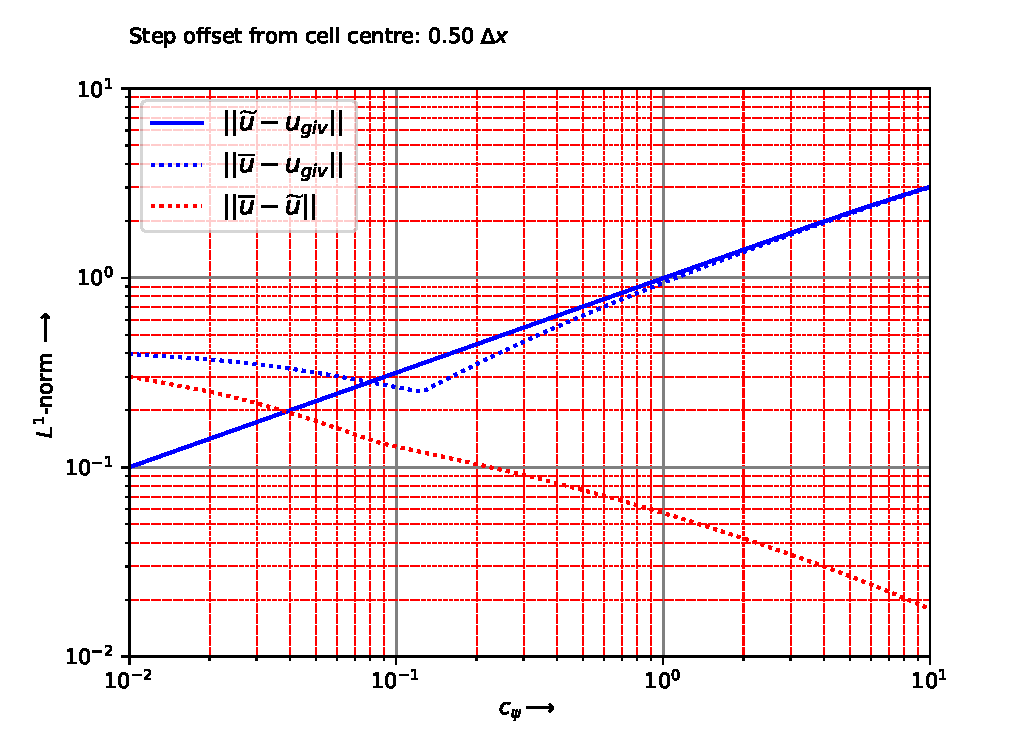
\includegraphics[width=\textwidth]{figures/regul_1d_step_at=0.5_dx50.0.pdf}
    \caption{Step defined with an of set of  0.5 $\Delta x$ from cell centre, thus defined at cell face.\label{fig:L1_norm_dx_offset_0.5dx}}
\end{subfigure}
\caption{Several plots of $L^1$-norm for different locations of the step.}
% Python script: reg_1d_step_less_error_when_more_smoothing.py
\end{figure}

As seen from these figures.
When choosing  $c_{\Psi} > 4$ then the $L^1$-norm of $\abs{|\overline{u} - \widetilde{u}|}_{1}$ is for all locations of the step smaller then $\num{2e-2}$ (red dotted lines in the plots).
Also the blue and blue dotted line are close together for $c_{\Psi}>4$.
That is the region in which we want to have the discetisation because there is the difference between the piecewise linear numerical solution $\overline{u}$ and the regularized solution $\widetilde{u}$ is independent of the location of the step, given by the function $u_{\it{giv}}$.

We also see that the dotted blue line is completely above the blue line if the step is located at the cell centre and with an offset of $0.3\Dx$ (see \autoref{fig:L1_norm_dx_offset_0.0dx} and \autoref{fig:L1_norm_dx_offset_0.3dx})
and it is partly below the blue line if the offset of the step is located at $0.5\Dx$ (\autoref{fig:L1_norm_dx_offset_0.5dx}).
The dotted blue line has also a sharp bend at the location where $c_{\Psi}=0.125$. These approximations are presented in the \autoref{fig:step_dx_offset_0.0dx}, \autoref{fig:step_dx_offset_0.3dx} and \autoref{fig:step_dx_offset_0.5dx}.
As seen from these plot the piecewise linear approximation shown in   \autoref{fig:step_dx_offset_0.5dx} is closer to the Heaviside function as the other two approximations.
\begin{figure}[H]
\begin{subfigure}{0.5\textwidth}
    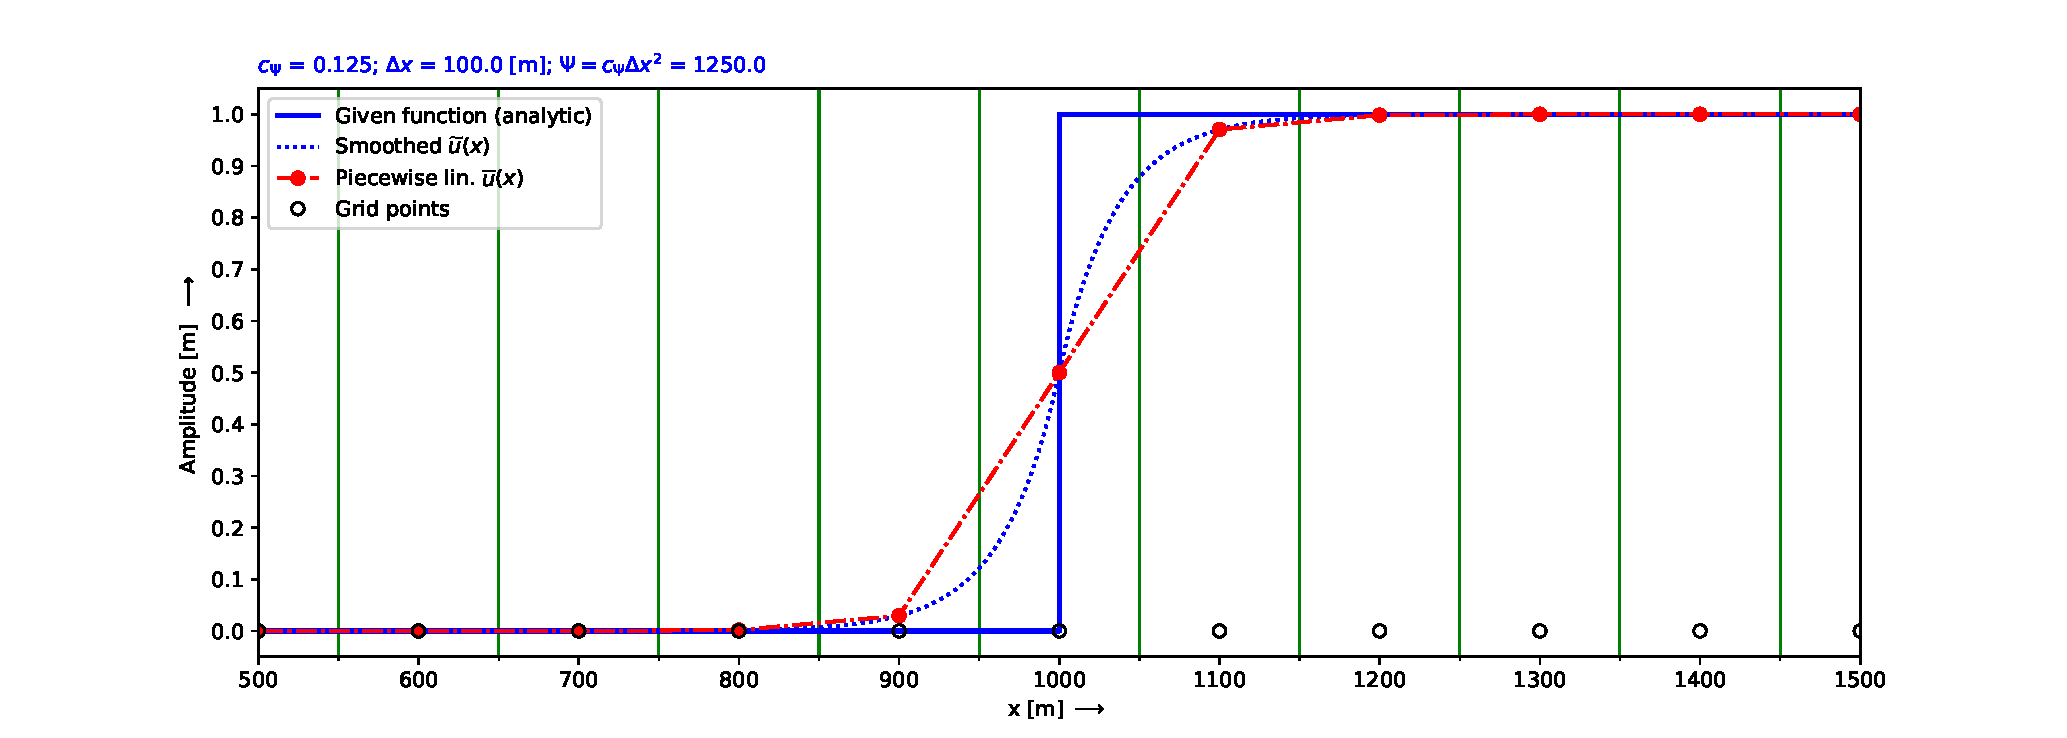
\includegraphics[width=\textwidth]{figures/regul_1d_step_at_0.00_function_dx100.0_cpsi0.125.pdf}
    \caption{Step defined at cell centre.\newline\phantom{text}\label{fig:step_dx_offset_0.0dx}}
\end{subfigure}
\begin{subfigure}{0.5\textwidth}
    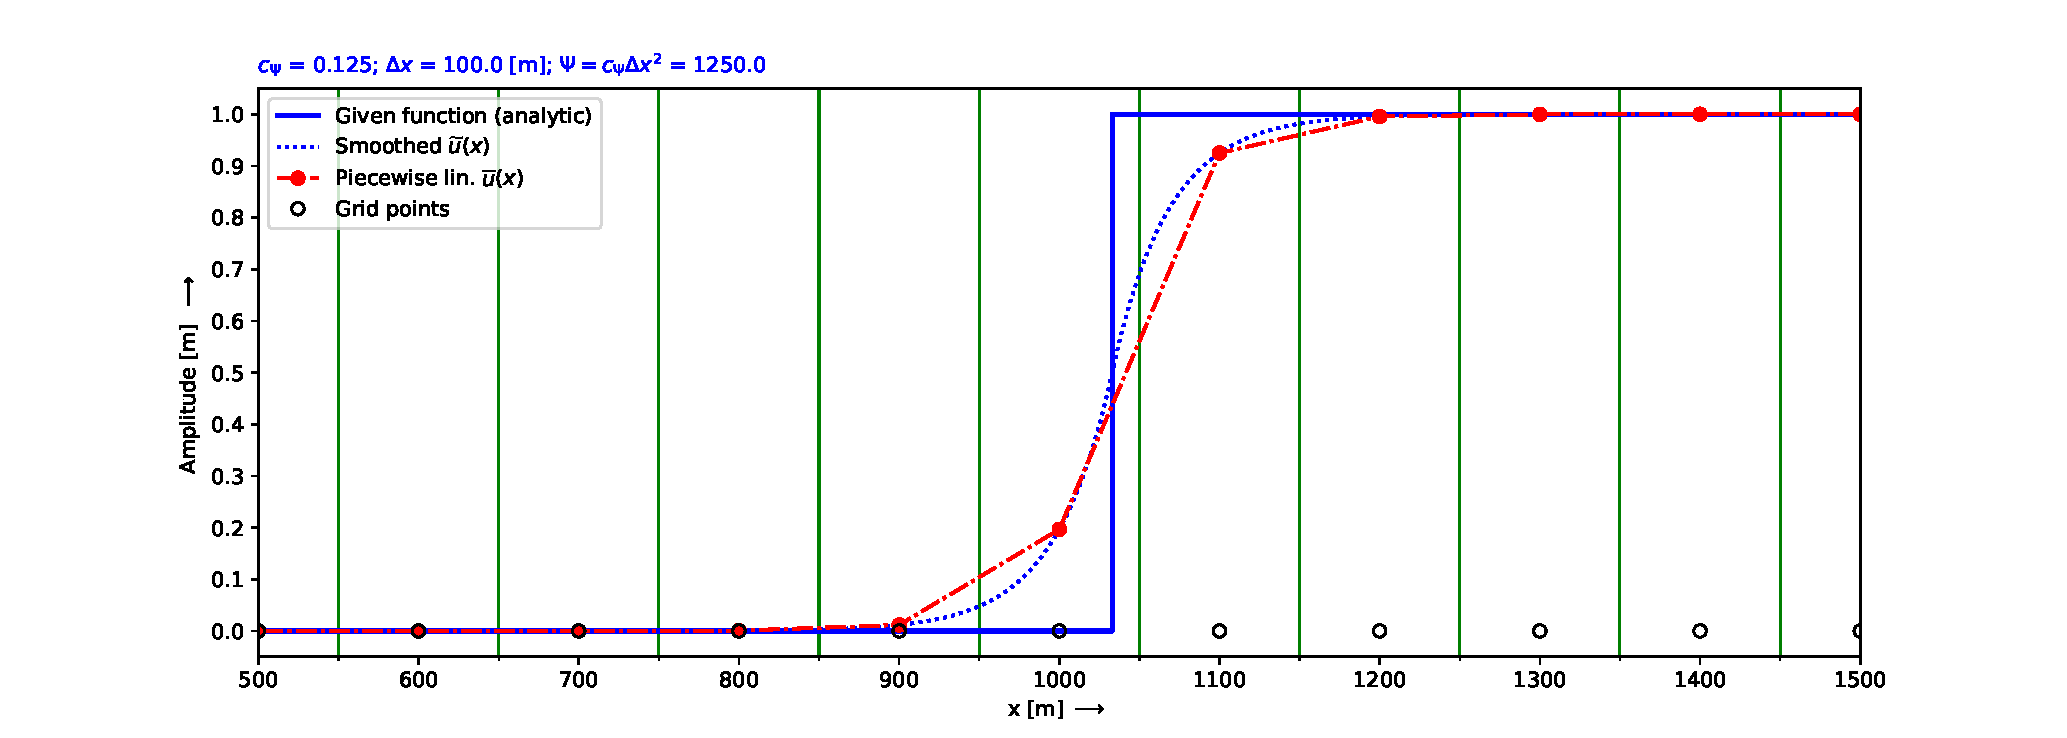
\includegraphics[width=\textwidth]{figures/regul_1d_step_at_0.33_function_dx100.0_cpsi0.125.pdf}
    \caption{Step defined with an of set of  0.3 $\Delta x$ from cell centre.\label{fig:step_dx_offset_0.3dx}}
\end{subfigure}
\newline
\begin{subfigure}{0.5\textwidth}
    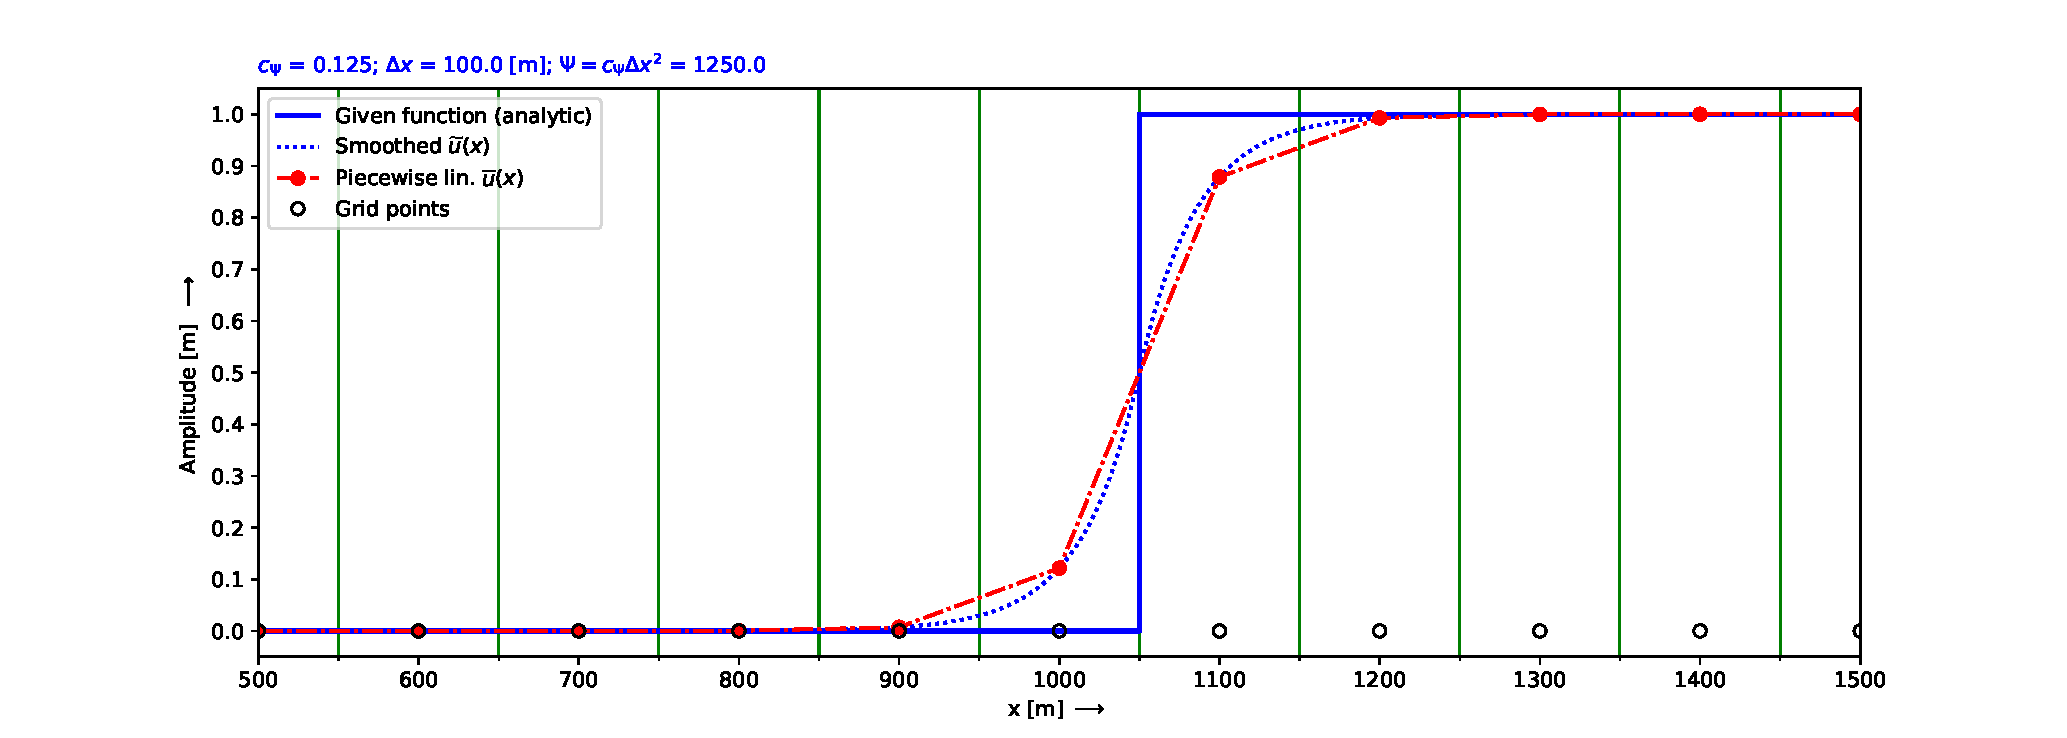
\includegraphics[width=\textwidth]{figures/regul_1d_step_at_0.50_function_dx100.0_cpsi0.125.pdf}
    \caption{Step defined with an of set of  0.5 $\Delta x$ from cell centre, thus defined at cell face.\label{fig:step_dx_offset_0.5dx}}
\end{subfigure}
\caption{Several plots of the piecewise linear approximation ($\overline{u}$) of the Heaviside function compared to the regularized function ($\widetilde{u}$).}
% Python script: reg_1d_step_less_error_1d_step_function.py
\end{figure}
